\question %3
\emph{Implémentez sous MATLAB ce modèle linéaire continu,
et calculez la solution correspondant aux données fournies sur icampus
(utilisez la fonction \texttt{linprog}).
Commentez l'allure de la solution obtenue.}

Notre implémentation se trouve dans le fichier \texttt{question3.m}.
Il nous parait important d'expliquer en quelques mots le r\^ole
de la fonction \texttt{kron}.
Celle-ci effectue le produit tensoriel de Kronecker entre deux matrices.
C'est-à-dire que pour \texttt{kron(A,B)},
chaque élément de $A$ multiplie la matrice $B$.
En l'utilisant de manière appropriée avec des matrices nulles et diagonales,
on peut effectuer un remplissage des matrices des contraintes très efficace.

Un exemple d'utilisation de cette fonction pour remplir la matrice
des contraintes se trouve dans l'annexe~\ref{app:kron}.

Les résultats obtenus sont représentés graphiquement
à la figure~\ref{fig:grapheProduction}.
Comme on pouvait s'y attendre, la solution optimale utilise presque chaque
semaine au maximum la ressource la moins chère,
en l'occurrence la production par les ouvriers payés au salaire normal.
On observe également que la solution optimale constitue un stock dans la première partie de la planification pour faire face au pic de demande
situé entre les semaines 5 et 8.
La demande est particulièrement importante à la semaine 7,
et on voit que notre stock constitué s'épuise totalement lors de cette semaine.
On commence également à avoir recours au retard.

+ QQ OBSERVATIONS SUR LE COMPORTEMENT DU SOLVER LINPROG?

Notre fonction MATLAB relative à cette question est \texttt{question3.m}. Nous vous invitons à taper \texttt{help question3} en ligne de commande afin de savoir comment interagir avec celle-ci.

\begin{figure}[H]
  \begin{center}
    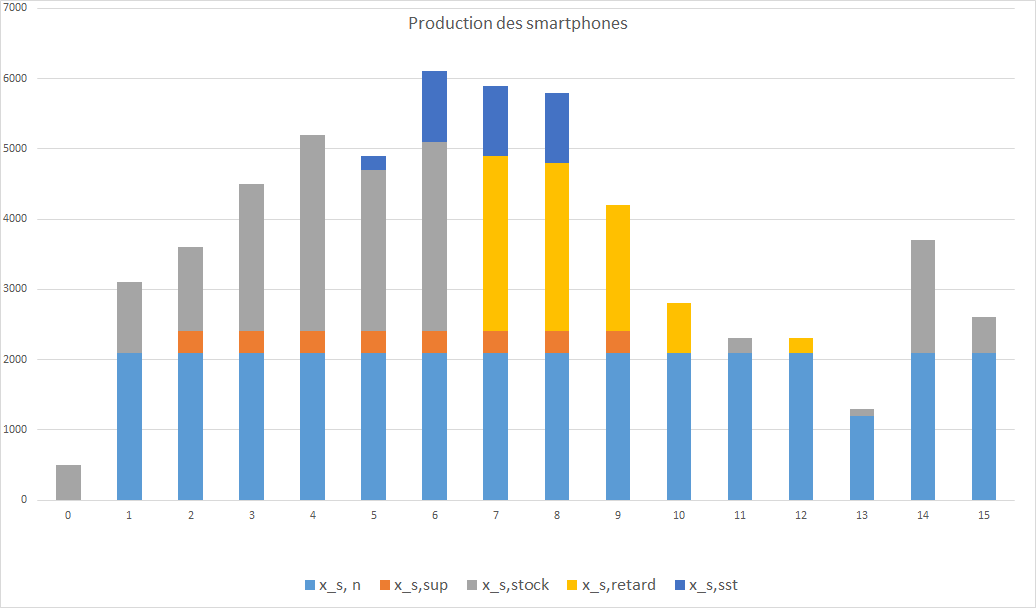
\includegraphics[scale = 0.8]{img/grapheProduction.png}
	  \caption{Répartition du moyen de production des smartphones en fonction des semaines.}
	  \label{fig:grapheProduction}
  \end{center}
\end{figure}
